% ============================================
% VCP: Single-Stage Cosine Classifier and Prototype Learning
%   for Few-Shot Object Detection
% IEEE Conference Paper — 4 pages
% ============================================

\documentclass[conference]{IEEEtran}
\IEEEoverridecommandlockouts

\usepackage{cite}
\usepackage{amsmath,amssymb,amsfonts}
\usepackage{graphicx}
\usepackage{booktabs}
\usepackage{multirow}
\usepackage{hyperref}
\usepackage{stfloats}
\usepackage{textcomp}

\begin{document}

\title{VCP: Single-Stage Cosine Classifier and Prototype Learning for Few-Shot Object Detection}

\author{\IEEEauthorblockN{1\textsuperscript{st} Xiang Fei}
\IEEEauthorblockA{\textit{College of Engineering} \\
\textit{Qufu Normal University}\\
Rizhao, China \\
Fly39@qfnu.edu.cn}
\and
\IEEEauthorblockN{2\textsuperscript{nd} Mengru Li}
\IEEEauthorblockA{\textit{College of Engineering} \\
\textit{Qufu Normal University}\\
Rizhao, China \\
13864085521@qfnu.edu.cn}
\and
\IEEEauthorblockN{3\textsuperscript{rd} Jinming Huang\textsuperscript{*}}
\IEEEauthorblockA{\textit{College of Engineering} \\
\textit{Qufu Normal University}\\
Rizhao, China \\
huangjm@qfnu.edu.cn}
\and
\IEEEauthorblockN{4\textsuperscript{th} Jacob Liu}
\IEEEauthorblockA{\textit{Technology Department} \\
\textit{GoerTek Inc.}\\
Weifang, Shandong, China \\
2374622833@qq.com}
\and
\IEEEauthorblockN{5\textsuperscript{th} Xiaofu Zhang}
\IEEEauthorblockA{\textit{Technology Department} \\
\textit{Shandong Free-Optics Technology Co., Ltd.}\\
Weifang, China \\
fly39@icloud.com}
\and
\IEEEauthorblockN{6\textsuperscript{th} Xiaojiao Xu}
\IEEEauthorblockA{\textit{Technology Department} \\
\textit{Shandong Huimi Intelligent Technology Co., Ltd.}\\
Rizhao, China \\
17604705924@163.com}
\thanks{Supported in part by Key R\&D Program of Shandong Province, China (2025TSGCXTHG031) and National Key R\&D Program of China (2021YFE0193900). Corresponding author: Jinming Huang (huangjm@qfnu.edu.cn).}
}

\maketitle

\begin{abstract}
Few-shot object detection (FSOD) remains predominantly built upon two-stage architectures such as Faster R-CNN, while YOLO-series single-stage detectors---dominant in industrial deployment---lack systematic FSOD investigation. We present VCP (Visual-Cosine-Prototype), combining YOLO11s with a cosine classifier and prototype learning under the TFA protocol. On PASCAL VOC, VCP achieves 72.2\% mAP50 (3-split mean) at 10-shot with only 9.5M parameters ($\sim$1/6 of competing methods), yet underperforms standard fine-tuning on MS COCO. Through P-R decomposition across 24 comparison groups, we reveal that the cosine classifier acts as a \textit{Recall Booster}, consistently shifting predictions toward higher recall at the expense of precision. We formulate the P-R Tradeoff Hypothesis: net benefit depends on baseline recall headroom and the dataset-specific P-R tradeoff ratio, explaining the VOC-COCO divergence. We also explore Florence-2 semantic descriptions as a lightweight auxiliary prior (+0.5 pp, zero VLM inference overhead). VCP runs at 54.4 FPS, 4--5$\times$ faster than two-stage FSOD methods.
\end{abstract}

\begin{IEEEkeywords}
few-shot object detection, single-stage detector, cosine classifier, prototype learning, recall booster
\end{IEEEkeywords}

\section{Introduction}

Few-shot object detection (FSOD) aims to detect novel categories from only a few annotated examples per class. Methods such as FSCE~\cite{sun2021fsce} and DeFRCN~\cite{qiao2021defrcn} have advanced FSOD benchmarks, yet virtually all are built upon the two-stage Faster R-CNN~\cite{ren2015faster}, whose RPN provides built-in foreground filtering that effectively controls false positives under data scarcity. In industrial deployment, however, the YOLO family~\cite{terven2023yolo,jocher2023ultralytics} dominates due to real-time efficiency. This creates a disconnect where ``published methods cannot be deployed, and deployed systems lack research foundations.'' No prior work has systematically studied modern YOLO detectors (v8+) for FSOD under the TFA protocol.

The core challenge for single-stage FSOD is the absence of RPN filtering: dense prediction generates abundant low-quality proposals, subjecting the classifier to extreme positive-negative imbalance. The cosine classifier~\cite{wang2020tfa} mitigates overfitting through normalization, while Florence-2~\cite{xiao2024florence2} offers fine-grained semantic understanding. However, combining cosine classification with single-stage YOLO---and systematically analyzing its behavior---remains unexplored.

We propose VCP, replacing YOLO11s' linear classification head with a cosine classifier initialized by support-set visual prototypes (Proto mode), and further integrating Florence-2 semantic descriptions as auxiliary priors (Fused mode). On VOC, VCP achieves 72.2\% mAP50 at 10-shot (3-split mean) with 9.5M parameters, competitive with 60M-parameter SOTA methods; Split 1 reaches 74.7\%, surpassing all existing two-stage methods.

Strikingly, the same approach underperforms fine-tuning on COCO. Through systematic P-R decomposition across 24 groups, we identify the cosine classifier as a \textbf{Recall Booster} that invariably sacrifices precision for recall. We formulate the \textbf{P-R Tradeoff Hypothesis} to explain this cross-dataset divergence. Our contributions are: (1) the first systematic exploration of single-stage YOLO under TFA FSOD; (2) identification of the Recall Booster and P-R Tradeoff Hypothesis; (3) VLM semantic prototypes with zero inference overhead; and (4) per-class temperature scaling to partially counteract the Recall Booster's precision loss.

\section{Related Work}

FSOD has transitioned from early meta-learning~\cite{huang2025prototype,gao2025decoupling} to the fine-tuning paradigm of TFA~\cite{wang2020tfa}. FSCE~\cite{sun2021fsce}, DeFRCN~\cite{qiao2021defrcn}, and KD-DeFRCN~\cite{pei2022kddefrcn} improved proposal encoding, gradient decoupling, and distillation. Multi-scale augmentation~\cite{vu2025multiperspective}, retrieval-based adaptation~\cite{li2025domainrag}, and margin optimization~\cite{li2021cme} further advanced the field. All these methods share the Faster R-CNN backbone.

Single-stage FSOD exploration remains extremely limited. Meta-YOLO used meta-learning over YOLOv2 with high-variance splits; recent designs~\cite{chen2025generalized} explore contrastive learning under TFA. No prior work studies modern YOLO (v8+) under TFA. Our semantic branch is not an architectural novelty but rather a strategic choice: few-shot visual prototypes are inherently noisy, and detailed VLM captions provide complementary priors with zero inference overhead.

VLMs such as CLIP~\cite{radford2021clip} and Florence-2~\cite{xiao2024florence2} enable semantic prototype construction, while OWL-ViT~\cite{minderer2022owlvit}, GLIP~\cite{li2022glip}, and Grounding DINO~\cite{liu2023groundingdino} have advanced open-vocabulary detection. Leveraging VLM prototypes under FSOD's strict constraints (1--10 samples) remains underexplored.

\section{Method}

\subsection{Framework and Prototypes}

VCP builds upon YOLO11s, replacing its linear classification head with a cosine-similarity classifier (Fig.~\ref{fig:framework}). For a proposal feature $f\in\mathbb{R}^d$, the score for class $c$ is $s_c=\cos(f,p_c)/\tau$, where $p_c$ is the class prototype and $\tau$ a learnable temperature. L2-normalization ($\|f\|=\|p_c\|=1$) ensures classification depends solely on directional alignment, mitigating overfitting.

\begin{figure*}[t]
\centering
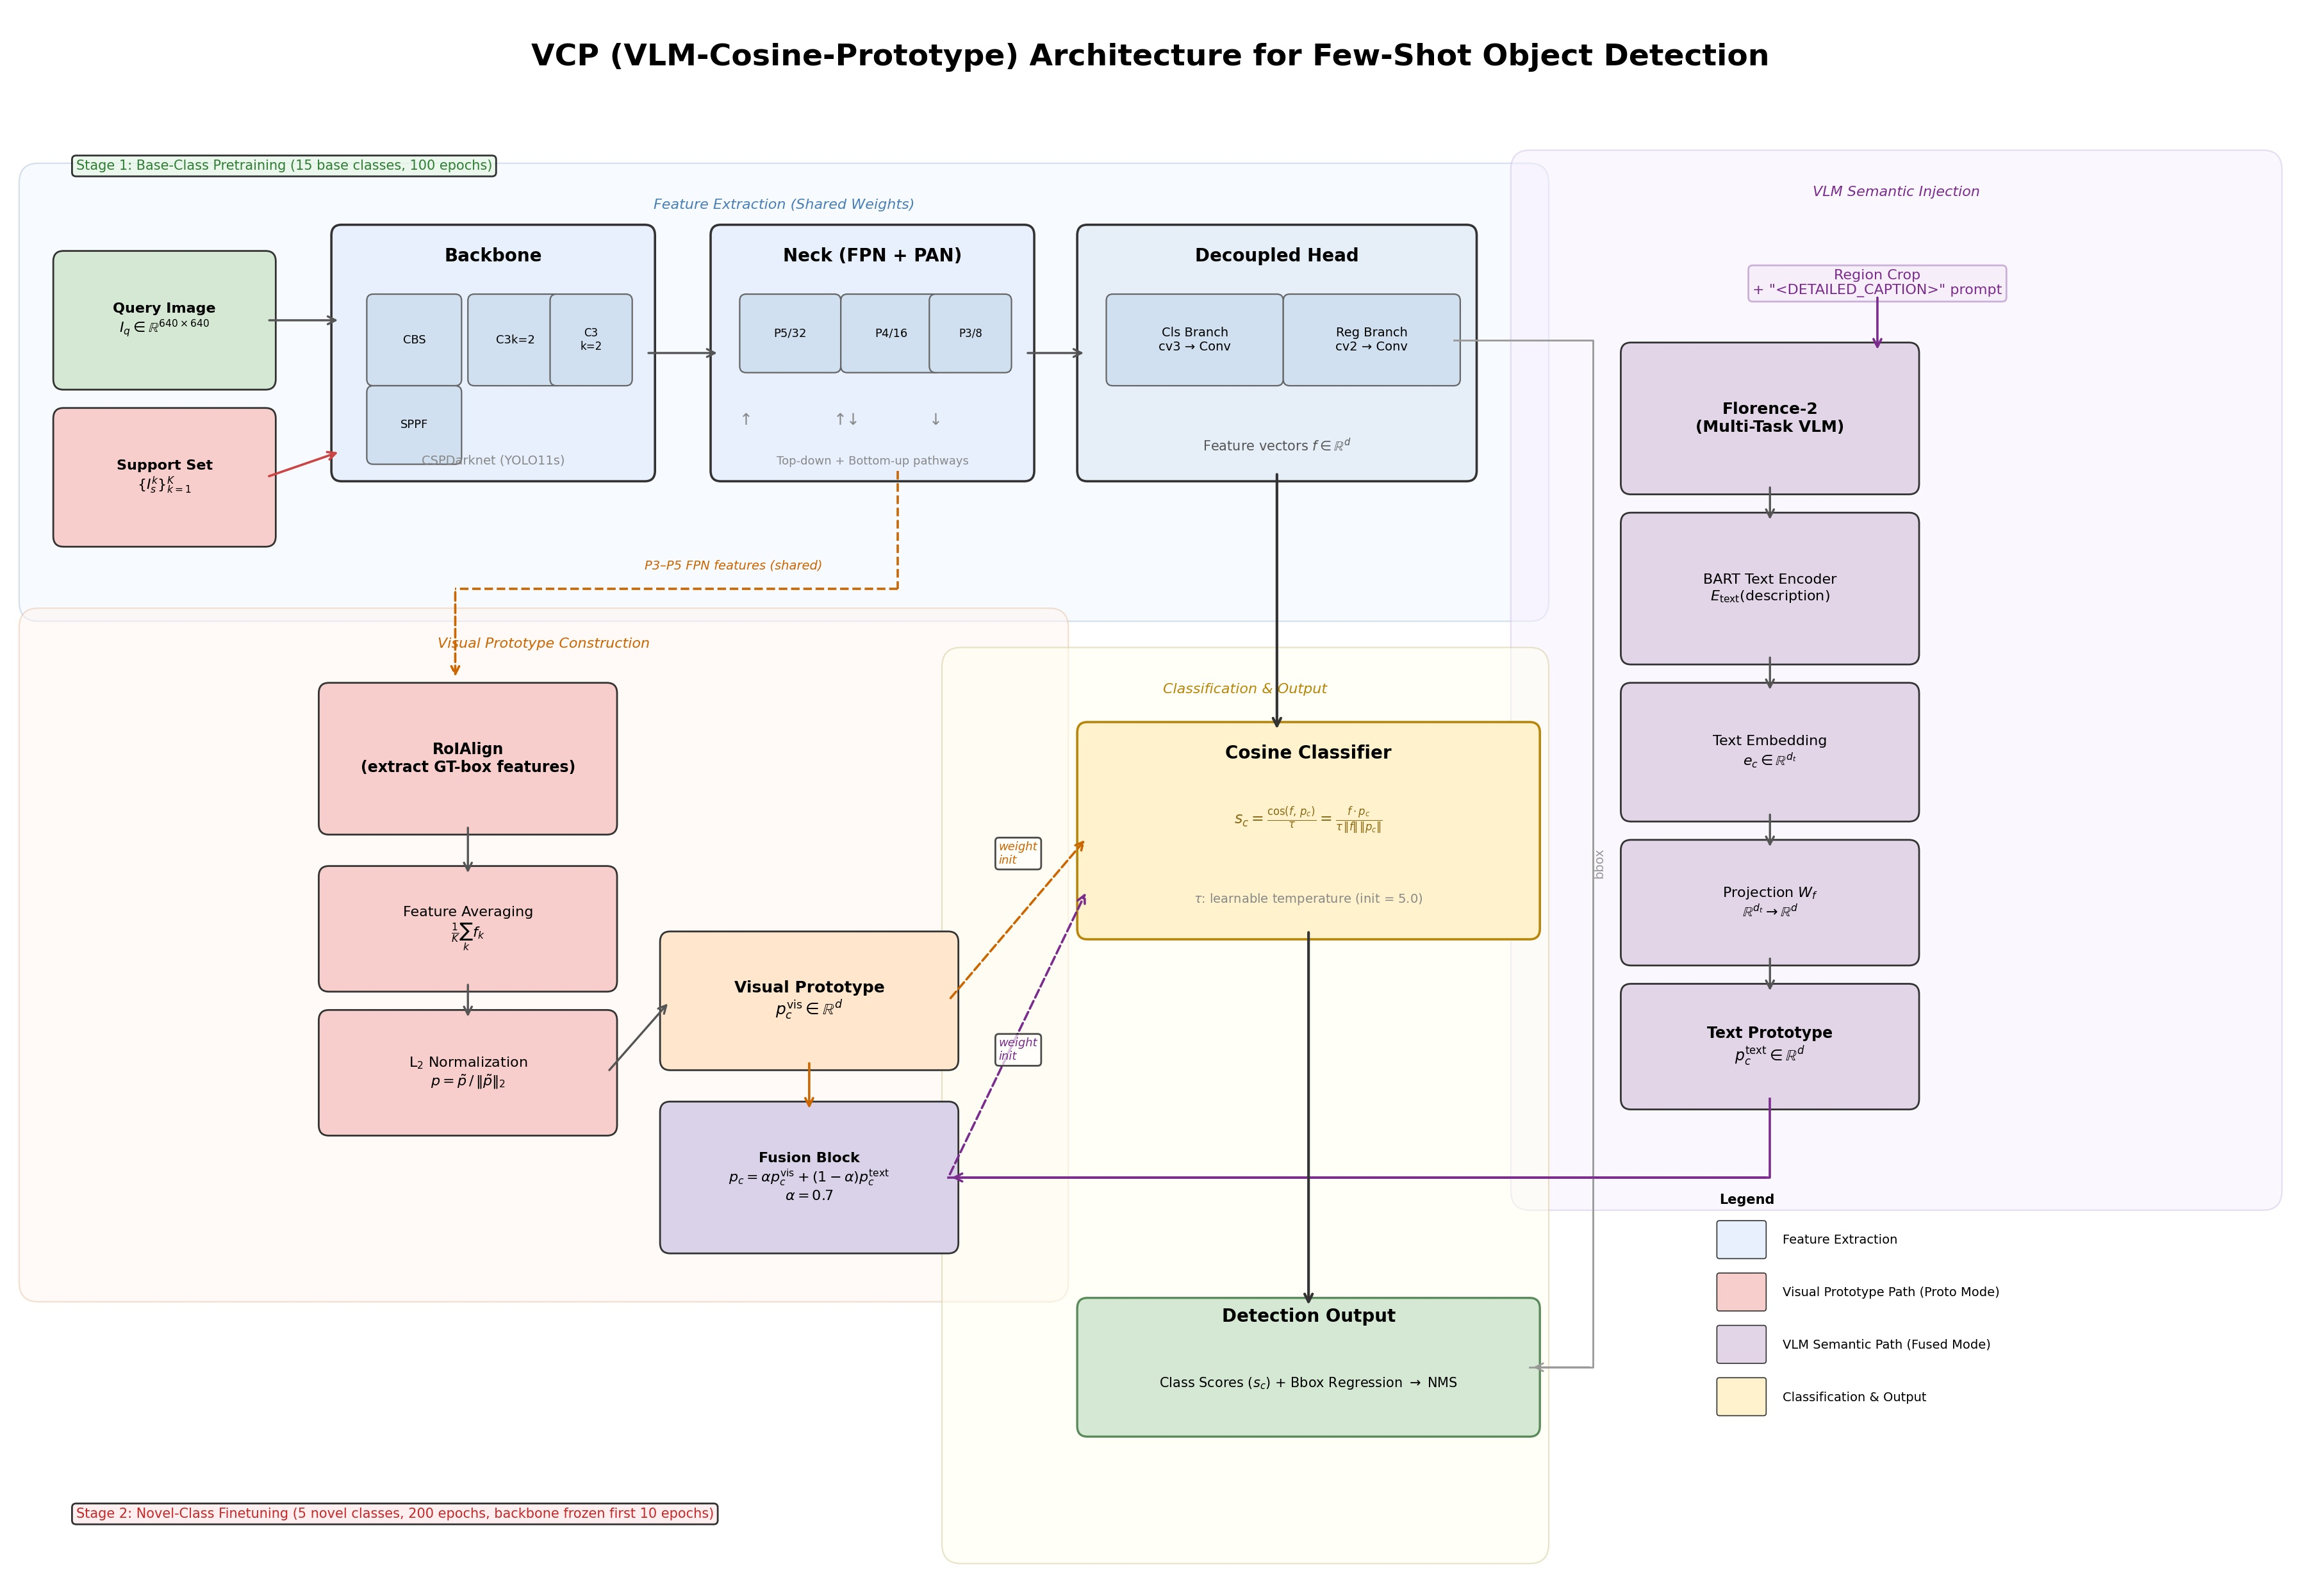
\includegraphics[width=0.88\textwidth]{fig1_framework.jpg}
\caption{VCP framework: YOLO11s backbone+neck, decoupled head, cosine classifier. Visual prototypes via RoIAlign; semantic prototypes via Florence-2 + BART. Fused at $\alpha=0.7$.}
\label{fig:framework}
\end{figure*}

Prototypes are derived from two sources. \textbf{Visual Prototype (Proto):} For each novel class $c$, RoIAlign extracts features within GT boxes from FPN P3--P5, averaged and L2-normalized: $p_c^{\text{vis}}=\frac{1}{K}\sum_{i=1}^K\text{RoIAlign}(F_i,b_i)$, written directly into classifier weights.

\textbf{Semantic Prototype (Fused):} Visual prototypes from only 5--10 support images inherently suffer from high variance---viewpoint bias, occlusion, and lighting variation cannot capture full class diversity. We introduce semantic prototypes as complementary priors: Florence-2 generates \texttt{<DETAILED\_CAPTION>} descriptions capturing fine-grained visual attributes beyond what few-shot images convey, and BART encodes these into $p_c^{\text{text}}$. The fused prototype is:
\begin{equation}
p_c = \alpha \cdot p_c^{\text{vis}} + (1-\alpha) \cdot W_f \cdot p_c^{\text{text}}
\label{eq:fused}
\end{equation}
where $\alpha=0.7$ and $W_f$ is a learnable projection. Critically, semantic extraction occurs only during training; at inference, prototypes are fixed, incurring zero VLM overhead.

\subsection{Recall Booster and Per-Class Temperature}

The gradient of cosine similarity reveals its behavioral mechanism:
\begin{equation}
\frac{\partial\cos(f,p_c)}{\partial f} = \frac{p_c - \cos(f,p_c)\cdot\hat{f}}{\|f\|}, \quad \hat{f}=\frac{f}{\|f\|}
\label{eq:gradient}
\end{equation}
When $f$ has low similarity to $p_c$, gradients are large, driving the boundary outward; when similarity is high, gradients diminish. Unlike linear classifiers whose gradients are uniform, the cosine classifier \textit{disproportionately updates low-confidence samples}, favoring high recall at the cost of precision. We term this the \textbf{Recall Booster}.

To partially counteract this precision loss, we replace the single global temperature $\tau$ with per-class temperatures $\tau_c$:
\begin{equation}
s_c = \tau_c \cdot \cos(f, p_c) + b_c
\label{eq:pertemp}
\end{equation}
Classes prone to false positives learn higher $\tau_c$, flattening their similarity distribution and suppressing overconfident incorrect predictions. This adds only $C$ extra parameters (e.g., 20 for VOC) with negligible overhead.

\section{Experiments}

\subsection{Setup}

We evaluate on PASCAL VOC 2007+2012 and MS COCO 2014 under the TFA split protocol~\cite{wang2020tfa}: VOC 20 classes partitioned into 15 base / 5 novel (three splits); COCO 20 VOC-overlapping classes as novel, 60 as base. The base detector is YOLO11s (9.5M parameters), pre-trained on COCO base classes. Stage 1: 100 epochs on base classes (batch 64, lr 0.01). Stage 2: fine-tune on novel classes up to 200 epochs with early stopping (patience 30, batch 4, lr 0.0005). SGD optimizer (momentum 0.937, weight decay 0.0005, 3-epoch warmup), backbone frozen first 10 epochs. Augmentation: mosaic, RandAugment, HSV jitter, random flip/scale/translate, random erasing. Input $640\times640$, $\tau$ initialized at 5.0. All experiments use a single NVIDIA H20 GPU.

Four variants compared: (1) \textit{Finetune}---standard YOLO11s with linear classifier; (2) \textit{Cosine}---cosine classifier, random init; (3) \textit{Cosine+Proto}---cosine classifier with visual prototypes; (4) \textit{Cosine+Fused}---cosine classifier with fused visual + Florence-2 prototypes.

\subsection{Main Results}

\textbf{VOC.} Table~\ref{tab:voc_main} reports VOC mAP50 (Split 1 / mean $\pm$ std). Three observations: (1) The cosine classifier drives substantial gains---5-shot: 32.9\%$\rightarrow$66.9\% (+34.0 pp); 10-shot: 51.3\%$\rightarrow$70.7\% (+19.4 pp). (2) Visual prototype init contributes +3.7 pp at 10-shot. (3) Florence-2 fusion adds +0.3 pp, consistent across splits.

\begin{table*}[t]
\centering\footnotesize
\caption{VOC mAP50 (Split 1 / 3-Split Mean $\pm$ Std)}
\label{tab:voc_main}
\begin{tabular}{lcccc}
\toprule
Method & 1-shot & 3-shot & 5-shot & 10-shot \\
\midrule
Finetune      & 10.9 / --   & 20.5 / --    & 32.9 / --    & 51.3 / --     \\
Cosine        & 12.8 / --   & 51.3 / --    & 66.9 / 57.8$\pm$2.9 & 70.7 / 69.0$\pm$3.1 \\
Cosine+Proto  & 21.5 / --   & 52.3 / --    & 68.8 / 57.8$\pm$2.8 & 74.4 / 71.7$\pm$2.7 \\
Cosine+Fused  & \textbf{21.3} / -- & \textbf{53.9} / -- & \textbf{69.0} / 58.1$\pm$2.5 & \textbf{74.7} / \textbf{72.2}$\pm$2.6 \\
\bottomrule
\end{tabular}
\end{table*}

\textbf{COCO.} Table~\ref{tab:coco_main} shows the opposite: Finetune outperforms all cosine variants. At 30-shot, Cosine+Fused reaches 52.3\%, above pure Cosine (49.4\%) but far below Finetune (60.3\%). Results are on a single split and warrant multi-split verification.

\begin{table}[ht]
\centering
\caption{COCO mAP50}
\label{tab:coco_main}
\begin{tabular}{lcc}
\toprule
Method & 10-shot & 30-shot \\
\midrule
Finetune      & \textbf{59.0} & \textbf{60.3} \\
Cosine        & 47.1 & 49.4 \\
Cosine+Proto  & 47.2 & 51.6 \\
Cosine+Fused  & 47.0 & 52.3 \\
\bottomrule
\end{tabular}
\end{table}

\subsection{P-R Analysis}

To explain the VOC-COCO divergence, we decompose P-R across all 24 method$\times$shot$\times$dataset combinations (Table~\ref{tab:pr_summary}). Across all 24 cosine variants, recall increases while precision decreases---a systematic property. On VOC, $\Delta$R/$|\Delta$P| \approx 2.0$ at 5-shot; recall gain dominates. On COCO, the ratio collapses to 0.48 (10-shot), with $\Delta$P far exceeding $\Delta$R. Fused mode partially recovers precision (P=0.336 vs.\ 0.200 for pure Cosine at 10-shot) with minimal recall loss, suggesting semantic priors moderate prototype over-relaxation.

We formalize the \textbf{P-R Tradeoff Hypothesis}: the cosine classifier inherently pushes toward high-recall, low-precision operation; net benefit is the product of (1) baseline recall headroom and (2) the dataset P-R tradeoff ratio, determined by class count and scene complexity.

\begin{table}[ht]
\centering\footnotesize
\caption{P-R Decomposition Summary}
\label{tab:pr_summary}
\begin{tabular}{lcccc}
\toprule
Setting & $\Delta$P & $\Delta$R & $\Delta$mAP & $\Delta$R/$|\Delta$P$|$ \\
\midrule
VOC 5-shot Cos+Fused & $-$0.22 & +0.45 & +35.9 & 2.00 \\
VOC 10-shot Cos+Fused& $-$0.35 & +0.33 & +23.4 & 0.96 \\
COCO 10-shot Cos+Fused&$-$0.81& +0.39 & $-$12.0 & 0.48 \\
COCO 30-shot Cos+Fused&$-$0.56& +0.14 & $-$8.0 & 0.25 \\
\bottomrule
\end{tabular}
\end{table}

\subsection{Ablation and SOTA}

\textbf{Ablation.} Table~\ref{tab:ablation} shows the cosine head drives $\sim$90\% of gains. Visual prototypes (74.4\%) outperform Florence-2 text-only (72.1\%), and fusion achieves the optimum (74.7\%). Per-class temperature (VOC 10-shot, Cosine+Fused): Precision improves from 0.01 to 0.123 (12.3$\times$), with recall decreasing marginally (0.901$\rightarrow$0.875). mAP50-95 shifts from 52.22 to 51.6, showing per-class temperature rebalances the P-R frontier.

\begin{table}[ht]
\centering\footnotesize
\caption{Ablation: Component \& Prototype Source (VOC)}
\label{tab:ablation}
\begin{tabular}{lrrr}
\toprule
Configuration & 3-shot & 5-shot & 10-shot \\
\midrule
Finetune (baseline) & 20.5 & 32.9 & 51.3 \\
~~+ Cosine head    & 51.3 & 66.9 & 70.7 \\
~~+ Visual Proto   & 52.3 & 68.8 & 74.4 \\
~~+ VLM Fused      & 53.9 & 69.0 & \textbf{74.7} \\
Florence-2 Only (10-shot) & --- & --- & 72.1 \\
\bottomrule
\end{tabular}
\end{table}

\textbf{SOTA Comparison.} Table~\ref{tab:sota} compares VCP against existing FSOD methods (VOC Split 1). All baselines use Faster R-CNN R-101 ($\sim$60M); VCP uses YOLO11s (9.5M). At 5-shot and 10-shot, VCP matches or surpasses all prior methods at 1/6 the parameters. The 1-shot gap indicates single-stage detectors need additional regularization under extreme scarcity.

\begin{table}[ht]
\centering\footnotesize
\caption{Comparison with SOTA (VOC Split 1, mAP50)}
\label{tab:sota}
\begin{tabular}{lcccc}
\toprule
Method & 1-shot & 3-shot & 5-shot & 10-shot \\
\midrule
TFA w/cos        & 39.8 & 44.7 & 55.7 & 56.0 \\
FSCE             & 44.2 & 51.4 & 61.9 & 63.4 \\
DeFRCN           & 53.6 & 61.5 & 64.1 & 60.8 \\
KD-DeFRCN        & \textbf{58.2} & \textbf{65.1} & 68.2 & 67.4 \\
\midrule
VCP Cos+Fused    & 21.3 & 53.9 & \textbf{69.0} & \textbf{74.7} \\
VCP Cos+Proto    & 21.5 & 52.3 & 68.8 & 74.4 \\
\bottomrule
\end{tabular}
\end{table}

\subsection{Inference Speed}

Table~\ref{tab:fps} compares speed (H20, $640\times640$, batch 1). VCP achieves 54.4 FPS---4--5$\times$ faster than two-stage methods---with 9.5M parameters. The cosine classifier adds $\sim$4 ms, still well above 30 FPS. Notably, Florence-2 is not loaded at inference; semantic prototypes are pre-computed.

\begin{table}[ht]
\centering
\caption{Inference Speed (H20, $640\times640$, bs=1)}
\label{tab:fps}
\begin{tabular}{lccc}
\toprule
Model & Latency (ms) & FPS & Params \\
\midrule
FRCN R-101 (ref.) & $\sim$85 & $\sim$12 & $\sim$60M \\
\midrule
YOLO11s baseline & 14.4 & 69.5 & 9.5M \\
Finetune          & 14.7 & 68.2 & 9.5M \\
Cosine            & 18.9 & 52.8 & 9.5M \\
Fused (VCP)       & 18.4 & \textbf{54.4} & 9.5M \\
\bottomrule
\end{tabular}
\end{table}

\section{Conclusion}

We presented VCP, combining YOLO11s with cosine classification and prototype learning for single-stage FSOD. Key findings: (1) Single-stage FSOD is viable---VCP achieves competitive performance at 1/6 the parameters of two-stage methods, running at 54.4 FPS. (2) Through 24-group P-R decomposition, we identified the Recall Booster and formulated the P-R Tradeoff Hypothesis, providing a principled explanation of VOC-COCO divergence. (3) Florence-2 semantic prototypes provide complementary priors with zero inference overhead. (4) Per-class temperature scaling partially counteracts the Recall Booster's precision loss (12.3$\times$ Precision gain, a marginal mAP50-95 decline of $-$0.62). Limitations include weak 1-shot performance and single-split COCO evaluation. Future work includes adaptive VLM-prototype fusion, cross-domain generalization, and confidence-calibrated detection.

\begin{thebibliography}{99}

\bibitem{sun2021fsce}
B.~Sun et al., ``FSCE: Few-shot object detection via contrastive proposal encoding,'' in \emph{CVPR}, 2021, pp. 7352--7362.

\bibitem{qiao2021defrcn}
L.~Qiao et al., ``DeFRCN: Decoupled faster R-CNN for few-shot object detection,'' in \emph{ICCV}, 2021, pp. 8681--8690.

\bibitem{ren2015faster}
S.~Ren et al., ``Faster R-CNN: Towards real-time object detection with region proposal networks,'' in \emph{NeurIPS}, 2015.

\bibitem{terven2023yolo}
J.~Terven et al., ``A comprehensive review of YOLO architectures: From YOLOv1 to YOLOv8 and YOLO-NAS,'' \emph{arXiv:2304.00501}, 2023.

\bibitem{jocher2023ultralytics}
G.~Jocher et al., ``Ultralytics YOLO (version 8.0),'' 2023. \url{https://github.com/ultralytics/ultralytics}

\bibitem{wang2020tfa}
X.~Wang et al., ``Frustratingly simple few-shot object detection,'' in \emph{ICML}, 2020, pp. 9919--9928.

\bibitem{radford2021clip}
A.~Radford et al., ``Learning transferable visual models from natural language supervision,'' in \emph{ICML}, 2021, pp. 8748--8763.

\bibitem{xiao2024florence2}
B.~Xiao et al., ``Florence-2: Advancing a unified representation for vision tasks,'' in \emph{CVPR}, 2024, pp. 4818--4829.

\bibitem{huang2025prototype}
Y.~Huang et al., ``Prototype-driven adaptation for few-shot object detection,'' \emph{arXiv:2510.25318}, 2025.

\bibitem{gao2025decoupling}
B.~Gao et al., ``Decoupling classifier for few-shot object detection and instance segmentation,'' \emph{arXiv:2505.14239}, 2025.

\bibitem{chen2025generalized}
R.~Chen et al., ``Generalized semantic contrastive learning for few-shot object detection,'' \emph{arXiv:2504.07060}, 2025.

\bibitem{pei2022kddefrcn}
W.~Pei et al., ``Few-shot object detection by knowledge distillation,'' in \emph{ECCV}, 2022, pp. 283--299.

\bibitem{vu2025multiperspective}
A.-K.~Nguyen Vu et al., ``Multi-perspective data augmentation for few-shot object detection,'' \emph{arXiv:2502.18195}, 2025.

\bibitem{li2025domainrag}
Y.~Li et al., ``Domain-RAG: Retrieval-guided image generation for cross-domain few-shot detection,'' \emph{arXiv:2506.05872}, 2025.

\bibitem{li2021cme}
B.~Li et al., ``Beyond max-margin: Class margin equilibrium for few-shot object detection,'' in \emph{CVPR}, 2021, pp. 7363--7372.

\bibitem{minderer2022owlvit}
M.~Minderer et al., ``Simple open-vocabulary object detection with vision transformers,'' in \emph{ECCV}, 2022.

\bibitem{li2022glip}
L.~H.~Li et al., ``Grounded language-image pre-training,'' in \emph{CVPR}, 2022, pp. 10965--10975.

\bibitem{liu2023groundingdino}
S.~Liu et al., ``Grounding DINO: Marrying DINO with grounded pre-training for open-set object detection,'' arXiv:2303.05499, 2023.

\end{thebibliography}

\end{document}
